\section{Recursive Systematic Convolutional Codes:Review}
\label{sec2}

An $(n,k)$ RSC code is a convolutional code generated by using feedback shift registers which has its input bits as part of the codeword. At each time instant it receives an input of $k$ bits and outputs $n$ bits. The output bits are determined by the generator function, which may be written in $D$ notation as  $\Big[1 ~\frac{F(D)}{B(D)}\Big]$. Given the systematic nature of the RSC code, we only focus on the parity part of the RSC code and write the generator function simply as $\Big[\frac{F(D)}{B(D)}\Big]$ where $F(D)$ and $B(D)$ represent the feedfoward and feedback connections of the RSC encoder.  

It should be noted that the prescence of the feedback loop means that the code produced will have an infinite-length impulse response denoted $\bt$. A parameter which arises as a result of this infinite impulse response is know as the cycle length[5], denoted by $\tau$, which is defined as the length of the output cycle $\bp$ of an RSC encoder when the input is $(1~0~0~0~0~\cdots)$.The impulse response $\bt$ and by extension the cycle $\bp$ are unique for each RSC code. 

\begin{figure}[h]
\centering
		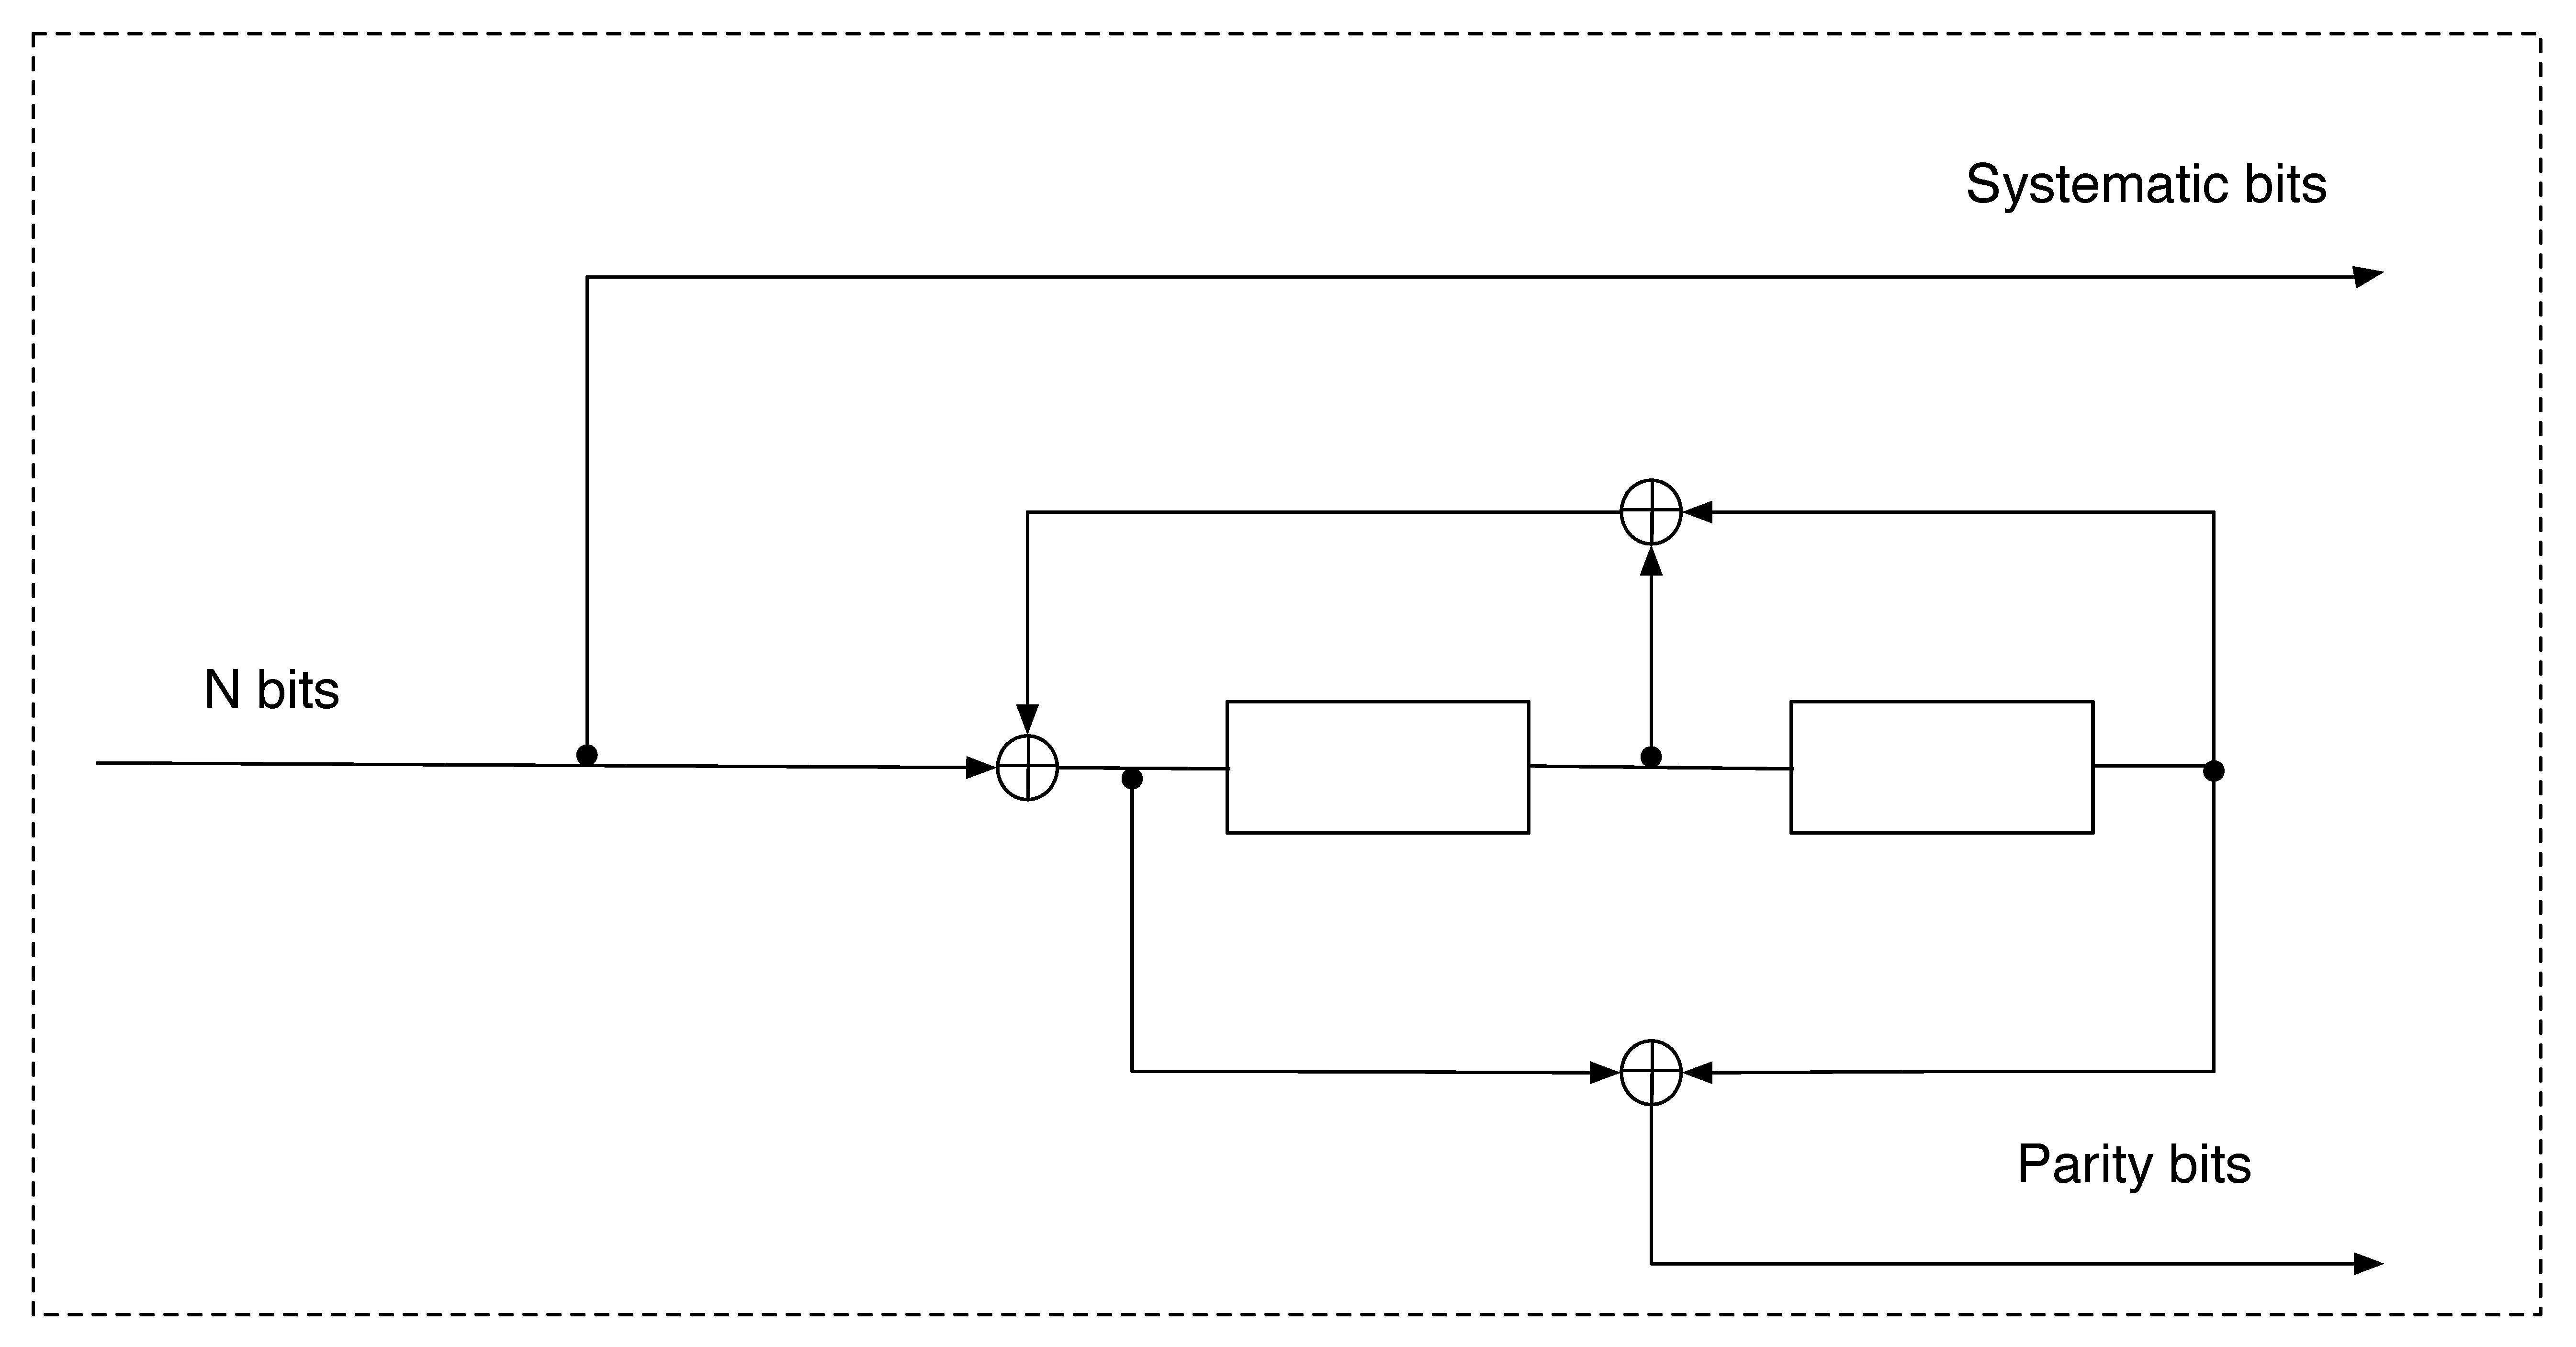
\includegraphics[width=0.45\textwidth]{RSCExample3.pdf}
		\caption{$[\frac{1+D^2}{1+D+D^2}]$  RSC Encoder}
		\label{fig1}
		\end{figure}
		
A RSC encoder is shown in Figure \ref{fig1}. Its generator function is given by $[\frac{1+D^2}{1+D+D^2}]$ which may be written as $5/7$ in octal form where $5 ~ \text{and} ~ 7$ correspond to the numerator and denomenator of the generator function respectively. 
 For the $5/7$ RSC code, $\bt=[1 1 1 0 1 1 0 1 1 0 ...]$ which gives us a cycle $\bp$ of $(1~1~0)$ and a cycle length $\tau =3$. 
 Also $k=1$ and $n=2$. Moving foward all examples and discussions relating to RSC codes will be done using the $5/7$ RSC code unless otherwise stated.
 %The knowledge of $\textbf{p}$ and $\tau$ will be used in deriving the method for determing which input messages generate low-weight parity bits. 